% !TEX TS-program = xelatex
% !TEX encoding = UTF-8 Unicode

% \documentclass[AutoFakeBold]{LZUThesis}
\documentclass[AutoFakeBold]{LZUThesis}
% \setCJKfamilyfont{Noto}{Noto Sans CJK SC}

\begin{document}
%=====%
%
%封皮页填写内容
%
%=====%

% 标题样式 使用 \title{{}}; 使用时必须保证至少两个外侧括号
%  如: 短标题 \title{{第一行}},  
% 	      长标题 \title{{第一行}{第二行}}
%             超长标题\tiitle{{第一行}{...}{第N行}}

\title{{基于Deep Koopman算子网络的}{非线性系统强化学习研究}}



% 标题样式 使用 \entitle{{}}; 使用时必须保证至少两个外侧括号
%  如: 短标题 \entitle{{First row}},  
% 	      长标题 \entitle{{First row}{ Second row}}
%             超长标题\entitle{{First row}{...}{ Next N row}}
% 注意:  英文标题多行时 需要在开头加个空格 防止摘要标题处英语单词粘连。
\entitle{{Deep Koopman Network Based}{ Reinforcement Learning of Nonlinear System}}

% \author{{\CJKfamily{Noto} \zihao{3} 许忞欢}}
\author{{许忞欢}}
\major{电子信息科学与工程}
\advisor{赵东东}
\college{信息科学与工程学院}
\grade{2020级}



\maketitle

%==============================%
% ↓ ↓ ↓ 诚信说明页 授权说明书
%==============================%

% 1. 可以调整签字的宽度,现在是40
% 2. 去掉raisebox的相关注释(注意上下大括号对应),可以改变-5那个数字调整签名和横线的上下位置

% 你的签名,signature.pdf 改为你的签名文件名,
\mysignature{
    % \raisebox{-5pt}{
    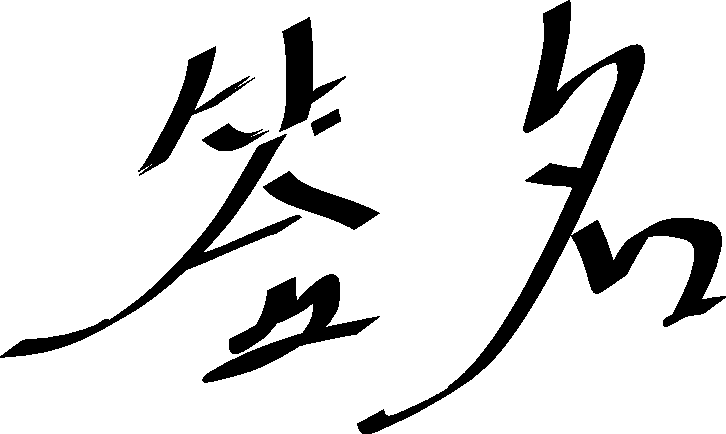
\includegraphics[width=40pt]{signature.pdf}
    % }
}
% 你手写的日期,signature.pdf 改为你的手写的日期文件名
\mytime{
    % \raisebox{-5pt}{
    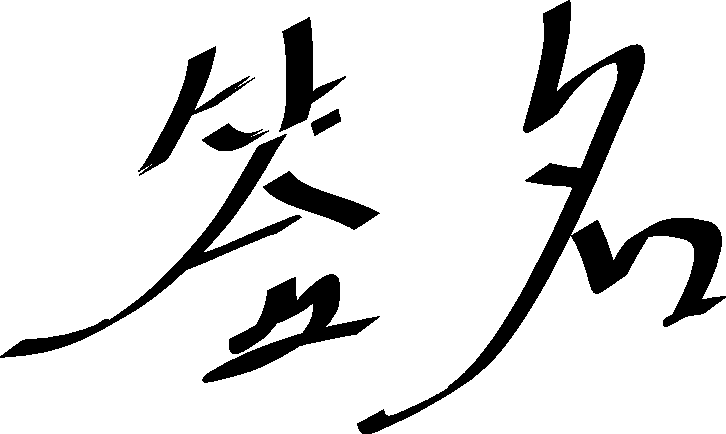
\includegraphics[width=40pt]{signature.pdf}
    % }
}
% 老师的手写签名,signature.pdf 改为老师的手写签名文件名
\supervisorsignature{
    % \raisebox{-5pt}{
    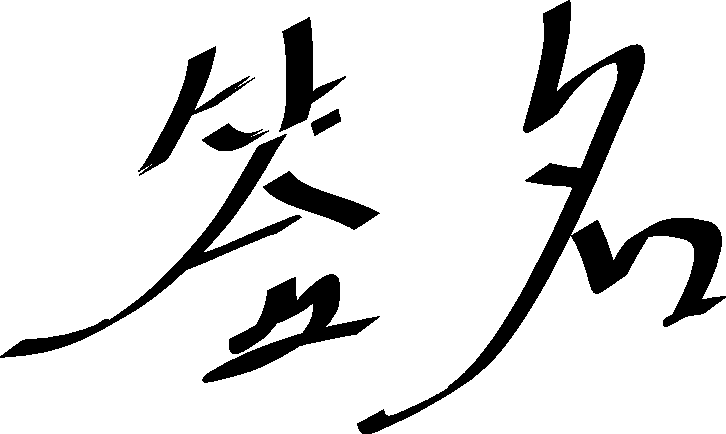
\includegraphics[width=40pt]{signature.pdf}
    % }
}
% 老师手写的时间,signature.pdf 改为老师的手写的日期文件名
\teachertime{
    % \raisebox{-5pSt}{
    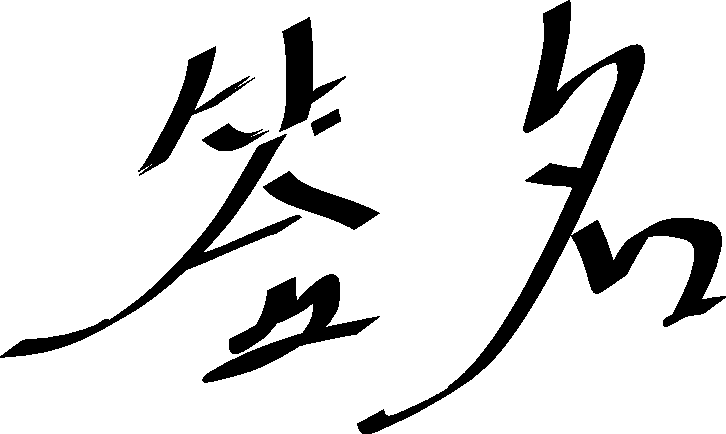
\includegraphics[width=40pt]{signature.pdf}
    % }
}
% 老师手写的成绩
\recommendedgrade{
    % \raisebox{-5pt}{
    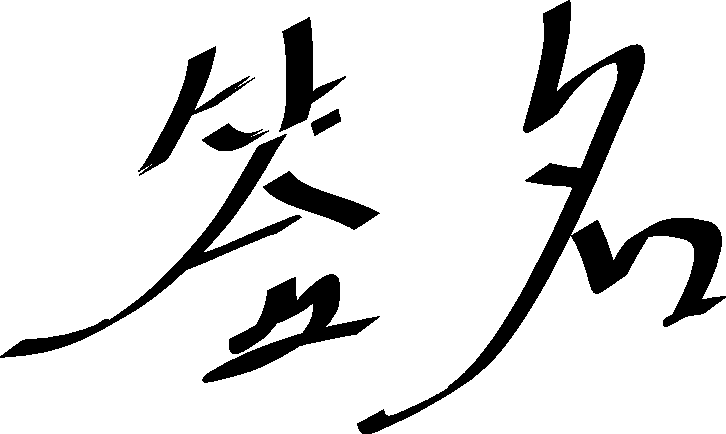
\includegraphics[width=40pt]{signature.pdf}
    % }
}

\makestatement

%==============================%
% ↑ ↑ ↑ 诚信说明页 授权说明书
%==============================%


%=====%
%论文(设计)成绩:注意2007的模板要求,成绩页在最后,2021要求成绩页在摘要前面
%=====%

% 下面这些注释掉可以去掉成绩、评语什么的
% \supervisorcomment{好好好}
%
%
% \committeecomment{优秀}
%
% \finalgrade{100}
% 上面这些注释掉可以去掉成绩、评语什么的


\frontmatter



%中文摘要
\ZhAbstract{我的摘要}{Koopman算子理论,深度神经网络,强化学习}


%英文摘要
\EnAbstract{My Abstract}{Koopman Operator Theory, Deep Neural Network, Reinforcement Learning}

%生成目录
\tableofcontents
% 下面这个包含图表目录
% \customcontent


% 部分同学需要专业术语注释表,* 表示不加入目录
% \chapter*{专业术语注释表}
% \begin{longtable}{lll}
%   \caption*{缩略词说明}\\
%   SS & Spread Spectrum & 扩展频谱 \\
%   PAPR & Peak to Average Power Ratio & 峰均比\\
%   DCSK & Differential Chaos Shift Keying &差分混移位键控\\
%   dasd & fdhfudw eqwrqw fasfasfs fewev wqfwefew &\tabincell{l}{太长了\\换行一下}\\
% \end{longtable}


%文章主体
\mainmatter

\chapter{\texorpdfstring{绪 \quad 论}{绪论}}

这是我的绪论\cite{tenne1992polyhedral}

\chapter{背景知识}
在本章中,首先讨论一下有关的背景理论与算法。介绍一下Koopman算子理论(Koopman Operator Theory),
并讨论Koopman算子对于重塑强化学习(Reinforcement Learning)中使用的马尔可夫决策过程(Markov Decision Process)的重要作用。
同时,对于Koopman算子理论与深度神经网络(Deep Neural Network)之间的关联。

\section{Koopman算子理论}
系统的强非线性是数据驱动建模和控制领域的核心问题之一,包括基于现代强化学习框架所做的工作。
Koopman算子理论[cite]为上述问题提出了一种解决方案。
在该理论中,非线性系统动力学可以在提升到无限维度希尔伯特空间时变为线性系统,并可以通过一组新的基底对于该线性系统进行观测。
升维工作已被证明对于线性化和简化某些具有挑战性的问题具有显著效果,这与机器学习领域中其他的类似努力相一致。

\subsection{非线性系统描述}
我们应该采用不同的形式对不同类型的系统中系统状态$x$进行描述。
假设系统为确定性自治系统,我可以采用下面的方式,将一个离散动力系统描述为
\begin{equation}
  \Dot{x} = F(x)
\end{equation}
其中,$\Dot{x}$表示下一个时刻的系统状态;或者,采取不同的方式,将一个连续动力系统描述为
\begin{equation}
  \frac{\mathrm{d}}{\mathrm{d}t} x(t) = f(x(t))
\end{equation}
而在处理实际问题是,我们通常考虑的是离散动力系统。
所以我们就可以将连续系统通过流映射算子(Flow Map Operator)归纳为一个离散系统,系统演化如下
\begin{equation}
  x(t + \tau) = F_\tau(x(t)) = x(t) + \int^{t + \tau}_t f(x(s)) \mathrm{d}s
\end{equation}

\subsection{Koopman算子与系统演化}
Koopman算子提供了解决非线性系统控制问题的一个新的着眼点。
在形式上,我们考虑一个实值向量测量函数$g: M \to \mathbb{R}$,且都由无限维希尔伯特空间的元素组成,其中$M$是一个流形。
通常,这个流形被认为是$L^\infty(X), \ X \subset \mathbb{R}^d$。
一般情况下,函数$g$被称为可观测函数。
Koopman算子理论中指出,Koopman算子$\mathcal{K}$和Koopman生成器$\mathcal{L}$
都是作用于上述观测函数$g$的无限维线性算子,在确定性系统中,有
\begin{subequations}
  \begin{align}
    \mathcal{K}g &= g \circ F \\
    \mathcal{L}g &= f \cdot \triangledown g
  \end{align}
\end{subequations}
Koopman生成器$\mathcal{L}$和Koopman算子有如下的关系
\begin{equation}
  \mathcal{L} g = \lim_{t \to 0} \frac{\mathcal{K}g - g}{t} = \lim_{t \to 0} \frac{g \circ F - g}{t}
\end{equation}

Koopman算子理论可以更广泛地应用于任何马尔可夫过程,但本文以随机性连续时间系统为例,此时,Koopman算子的定义如下:
\begin{align*}
  \mathcal{K} g &= \mathbb{E} (g(X) | X_0 = \cdot) \\
  \mathcal{L} g &= \lim_{t \to 0} \frac{\mathcal{K} g - g}{t}
\end{align*}

Koopman算子将测量函数$g$沿着路径$x$向前演化如下:
\begin{equation}
  \mathcal{K}_\tau g(x_t) := g(F_\tau(x_t)) = g(x_{t + \tau})
\end{equation}
其中$F$代表着系统的演化规律,或者更一般的,在随机自治系统中,$F$被如下定义为条件预测算子:
\begin{equation}
  \mathcal{K} g(x_t) = \mathbb{E}\left[g(X_{t + \tau}) | X_t = x_t\right]
\end{equation}
在上述离散系统算子中,普遍使用$\mathcal{K} := \mathcal{K}_1$,在本文中也照此用法。

% 值得注意的是,如上文所述,Koopman算子$\mathcal{K}$是一种作用于观测函数$g$的无限维线性算子,这意味着在由观测两系统的演化规律也将是线性的;

\subsection{Koopman算子本征函数}
上文提出,可观测函数$g$的观测,都存在于无限维的希尔伯特空间中(被称作观测空间),被如Koopman算子$\mathcal{K}$等无限维的算子推动沿着给定非线性动力学系统演化。
因此不难发现,我们可以应用Koopman算子理论研究,将对于非线性系统的研究,通过观测空间状态线性演化实现。

同时,由于难以捕捉无限维希尔伯特空间中所有可观测函数的演化,所以应该试图识别随着非线性系统动力学而线性演化的关键观测函数,
Koopman算子的本征函数就可以作为一组特殊的观测函数[cite]:
\begin{equation}
  \mathcal{K} \Phi (x_k) = \lambda \Phi(x_k) = \Phi(x_{k + 1})
\end{equation}
此时,本征函数就会成为观测空间的一组基底,由此,数学上,观测函数应当表示为这组基底的线性组合,如下:
\begin{equation}
  g(x) = \sum_{i = 1}^n a_i \Phi_i(x)
\end{equation}
此时,观测空间可被称为状态字典空间,同时,空间的基底可被称为字典函数

当前,从数据中挖掘信息并获得Koopman本征函数是现代动力学系统研究的主流方法,被称为数据驱动(Data-Driven)的Koopman算子。
由此,我们可以通过数据驱动的方式得到Koopman算子的本征函数,以得到非线性系统在高维空间中的全局线性表示。

此外,Koopman算子已经被广泛运用于受控系统。
在受控确定性离散时间系统中,我们有:
\begin{equation}
  x' = F(x, u)
\end{equation}
在受控连续时间系统中:
\begin{equation}
  \frac{\mathrm{d}}{\mathrm{d}t} = f(x(t), u(t))
\end{equation}

\section{强化学习}
强化学习(Reinforcement Learning)是机器学习(Machine Learning)和控制理论(Control Theory)的交叉领域,在强化学习中,智能体学习如何与复杂环境进行交互,并以获得更高的奖励为目标。
最近,深度强化学习(Deep Reinforcement Learning)被证明能够在若干项具有挑战性的任务中,实现人类水平或超人类的表现,包括玩电子游戏[cite]和策略游戏[cite]。
深度强化学习也越来越多地用于科学和工程应用,包括药物发现[cite]、机器人操作[cite],自动驾驶[cite]和无人机赛车[cite]、流体流量控制[cite]和融合控制[cite]。

\subsection{马尔可夫决策过程与贝尔曼方程}
马尔可夫决策过程是具有马尔可夫性质的随机过程。

随机过程是指研究对象是随时间演变的随机现象,在随机过程中,随机现象在某一时刻$t$的取值是一个向量随机变量,可以用$S_t$表示,所有可能的状态组成状态空间$\mathcal{S}$。
我们将已知所有历史状态$( S_1,\dots,S_t )$时,某一时刻$t$的状态$S_t$发生的概率用$P( S_{t + 1} | S_1,\dots,S_t )$表示。
而马尔可夫性质则表示,已知当前时刻状态$S_t$时,下一时刻状态$S_{t + 1}$仅与$S_t$有关,用$P( S_{t + 1} | S_t)$表示。而从前一状态经过随机进入下一状态的过程被称为状态转移。

在下文中,我们假设存在一个无限时域的马尔可夫决策过程。我们假设代理跟随随机策略$\pi(u | x)$,表示在已知状态$x$的情况下,采取某个特定动作$u$的可能性。
由此,在离散时间系统中,状态价值函数定义为:
\begin{equation}
  V^{\pi}(x) = \mathbb{E} \left[ \sum_{k = 0}^{\infty} \gamma^k r(x_k, u_k) |
  \pi, x_0 = x \right]
\end{equation}
其中,$r(x_k, u_k)$ 表示智能体得到的奖励;
$\gamma \in [0, 1]$ 表示折扣率,用于避免在无限时域时无限大的奖励。

在这里我们强调强化学习与控制领域的结合,所以本文中考虑使用线性二次最优控制问题。
线性二次最优控制是十分经典的控制领域问题,其中线性代表研究的系统动态可以用一组线性微分方程表示,
而其成本为二次泛函。
形式上,我们考虑有限时间长度,离散时间的LQR,假设离散时间线性系统:
$$
x_{k + 1} = A x_k + B u_k
$$
其性能指标为:
\begin{equation}
  c(x_k, u_k) = x_k^T Q x_k + u_k^T R u_k
\end{equation}
将系统线性二次性能指标的相反数作为智能体探索时的奖励:
\begin{equation}
  r(x_k, u_k) = - c(x_k, u_k)
\end{equation}
并改写贝尔曼方程可以得到:
\begin{equation}
  V^{\pi}(x) = \mathbb{E} \left[ \sum_{k = 0}^{\infty} - \gamma^k c(x_k, u_k) | \pi, x_0 = x \right]
\end{equation}

\subsection{演员-评委强化学习算法}
演员-评论家(Actor-Critic)强化学习算法是一种结合价值学习和策略学习的强化学习算法,
下面分三步介绍Actor-Critic强化学习算法。

首先介绍策略学习,在策略学习中,评价一个策略的方法是评估策略在环境中获得的回报的期望,此时目标函数为:
\begin{equation}
  J(\theta) = \mathbb{E}_S\left[ V_\pi (S) \right]
\end{equation}
其中,$V_\pi$代表状态价值函数,可以看到在这个目标函数中,
求得了状态价值函数有关状态的期望,所以只涉及到策略$\pi$的信息。
同时易知,这个目标函数该期望越大,表明该策略越好。

注意,在本文中,对于强化学习的研究只涉及深度强化学习,所以在这里使用深度神经网络的方式对策略网络进行测试。
所以,问题转化为如下的一个最大化问题:
\begin{equation}
  \max_{\theta} J(\theta)
\end{equation}
很明显,我们只需要使用梯度上升的方式迭代策略网络。
参数更新如下:
\begin{equation}
  \theta_{new} = \theta_{old} + \beta \cdot \triangledown_\theta J(\theta_{now})
\end{equation}
其中,$\beta$代表学习率,是需要调整的超参数,
梯度的具体表达式如下:
\begin{equation}
  \triangledown_\theta J(\theta_{now}) \triangleq \frac{\partial J(\theta)}{\partial \theta}
\end{equation}
以上算法被称为策略梯度

在策略学习中,我们想要得到的是当前策略能得到的价值函数,表示如下:
\begin{equation}
  V^\pi(s_t) = \mathbb{E} \left[ \sum_{k = t}^{N}
  \gamma^{k - t} \cdot r_k \right]
\end{equation}
在深度强化学习中,我们通过深度神经网络对价值进行近似,算法上,应该使得上述价值网络逼近真实价值函数。
一般使用时间差分(Temporal Differencial)算法来更新价值函数,根据贝尔曼方程:
\begin{equation}
  V^{\pi}(s_t) = \mathbb{E} \left[ r_t + \gamma V^\pi(s_{t + 1}) \right]
\end{equation}
等式左边为价值函数处于时间步$t$时对于价值的估计,等式右边是对于左边的一个无偏估计,
其中包含的$r_t$项使得等式右边比左边更加精确,所以应当使得价值网络逼近等式右边的值。
参数更新如下:
\begin{equation}
  Q^{new}(s_t, a_t) \leftarrow (1 - \alpha) Q^{now}(s_t, a_t) 
  + \alpha [ r_t + \gamma Q^{now}(s_{t + 1}, a_{t + 1}) ]
\end{equation}

最后,通过交替执行策略优化和价值优化,可以使得两者的性能逐渐同步提升。
策略网络可以获得更好的状态价值,价值网络可以实现更好的价值估计。
最后取用策略网络作为最优控制的策略函数就可以完成Actor-Critic算法在最优控制问题上的应用。



\chapter{Koopman算子辅助的最大熵强化学习}

贝尔曼方程及其连续形式汉密尔顿-雅可比-贝尔曼(Hamilton-Jacobi-Bellman)方程
在强化学习和控制理论中普遍存在。
然而,这些方程对于具有高维状态和非线性的系统来说,很快就变得难以处理。
本章将讨论数据驱动的Koopman算子与马尔可夫决策过程之间的联系,
并介绍借由此开发的两种新的强化学习算法来解决上述的问题。

技术上,我们可以利用Koopman算子技术将非线性系统提升到新的坐标中,其中动力学变得近似线性。
特别是,Koopman算子能够通过提升坐标中的线性动力学来捕获给定系统的价值函数的时间演化的期望。


\section{动作加权的Koopman张量}
我们现在关注如何通过Koopman算子在时间上推进观测基底函数,已知当前状态和动作,
也就是说,找到下面的一个映射:
\begin{equation}
  (x, u) \mapsto \phi(\dot x)
\end{equation}
我们要求观测函数近似地覆盖每个控制变量$u$的价值函数的有限维的Koopman不变子空间,因此存在矩阵$K^u \in \mathbb{R}^{d_x \times d_x}$,
使得$K^u \phi(x) = \phi(\dot x)$。

给定轨迹数据和状态字典空间$\phi$,为每个动作$u \in \mathcal{U}$构建如上的Koopman矩阵$K^u$。
为此,采取类似于SINDYc[cite]中描述的方法,其中状态和动作的字典空间用于预测下一个状态,
即$\Theta(x, u) \mapsto \dot x$
而这里的方法不同的地方有两点。
首先,不是试图预测下一个状态$x$,而是试图预测下一个字典函数值$\phi(x)$。
其次,为了让状态字典空间覆盖每个$u$的Koopman不变子空间,状态-动作字典在状态和动作上是可分离的。

这里,将状态-动作字典空间建模为乘法可分离的,就像$\psi(x) \circledtimes \phi(x)$
然后进一步假设存在线性映射$\psi(x) \circledtimes \phi(x) \mapsto \phi(\dot x)$。
下面描述如何为任何的$u$构建矩阵$K^u$。

令$\phi : \chi \mapsto \mathbb{R}^d_x$为状态的特征映射($\phi$的每一个分量都是一个可观测函数),
并且令$\psi: \mathcal{U} \mapsto \mathbb{R}^d_u$为控制动作的特征映射。
算法要求对于所有$u \in \mathcal{U}$得到Koopman算子$\mathcal{K}^u$的有限维逼近。
令$\mathcal{T}_{K} \in \mathbb{R}^{d_x \times d_x \times d_u}$为如图[ref]所示的三维向量。
对于任何$u$,如下定义:
\begin{equation}
  K^u[i, j] = \sum_{z = 1}^{d} \mathcal{T}_K (i, j, k) \phi(u)[z]
\end{equation}
形式上,$K^u$是沿着张量$\mathcal{T}$第三维的向量积,
同时,$K^u$作为对于Koopman算子$\mathcal{K}^u$的有限维近似。
因此,我们可以通过学习$\mathcal{T}_K$,来最小化字典函数$\phi$的误差:
\begin{equation}
  \min_{\mathcal{T}_K} \sum_{i = 1}^{N} || K^{u_i} \phi(x_i) - \phi(x_i') ||^2
\end{equation}
我们可以重写上述目标,使其成为一个规则的多变量线性回归问题,
将$\mathcal{T}_K$重新排列为一个大小为$\mathbb{R}^{d_x \times d_x d_u}$的二维矩阵。
令$M \in \mathbb{R}^{d_x \times d_x d_u}$,其中$M[i,:] \in \mathbb{R}^{d_x \cdot d_u}$
是堆叠二维矩阵$\mathcal{T}_K[i, :, :]$所得到的向量,如图[ref]所示。
令$\psi(u) \circledtimes \phi(x) \in \mathbb{R}^{d_x d_u}$为克罗内克积(Kronecker Product),所以有:
\begin{equation}
  K^u \phi(x) = M(\psi(u) \circledtimes \phi(x))
\end{equation}
从而,优化问题变成了常规的线性规划问题:
\begin{equation}
  \min_{M} \sum_{i = 1}^{N} || M(\phi(u) \circledtimes \phi(x_i)) - \phi(\dot x_i) ||^2
\end{equation}
只要我们计算出了$M$,我们就可以通过将$M$转换回为三维张量$\mathcal{T}_K$的方式
为任意系统执行的$u \in \mathcal{U}$得到标准的Koopman算子,
同时也得到了上述对$\mathcal{K}^u$的有限维近似$K^u \in \mathbb{R}^{d_x \times d_x}$

\section{最大熵强化学习最优控制问题}
考虑强化学习在最优控制领域的应用,在实践中最大的问题有以下两点:
首先,非常高的样本复杂度:使得智能体在探索中遇到困难;
其次,缓慢、不稳定的收敛过程:探索和利用的权衡是策略优化的重点,
特别是在最优控制中,不合适的样本利用和探索会使得策略过早的收敛到不良的局部最优值。
本文中使用最大熵强化学习算法,通过在训练目标中合理加入熵正则化项。
经过训练,策略可以最大化预期回报和熵。

\subsection{熵正则化}
粗略的说,熵是一个表示随机变量随机程度的量。
具体的说,如果一个随机变量的概率分布很集中,那么这个随机变量的熵就低;
如果一个随机变量的概率分布比较分散,那么这个随机变量的熵就高。

令$x$是具有概率质量密度函数的随机变量$P$。$H$的熵是根据$x$的分布得出的:
\begin{equation*}
  H(P) = \mathop{\mathbb{E}}_{x \sim P} \left[ - \log P(x) \right]
\end{equation*}
在熵正则强化学习中,代理在每个时间步获得与该时间步的策略熵成比例的奖金。
由此,目标策略变为:
\begin{equation}
  \pi^* = \arg \max_{\pi} \mathop{\mathbb{E}}_{\tau\sim\pi} 
  \left[ \sum_{t = 0}^{\infty} \gamma^t \left( r(s_t, a_t, s_{t + 1}) 
  + \alpha H(\pi(\cdot | s_t) \right) \right]
\end{equation}
其中$\alpha > 0$是权衡参数。我们现在可以在如上假定中给出略有不同的价值函数。
$V^{\pi}$更改为包含每个时间步的熵奖励:
\begin{equation}
  V^\pi = \mathop{\mathbb{E}}\limits_{\tau\sim\pi} 
  \left[ \sum_{t = 0}^{\infty} \gamma^t \left( r(s_t, a_t, s_{t + 1}) 
  + \alpha H(\pi(\cdot | s_t) \right) \left|\right. s_0 = s \right]
\end{equation}
$Q^\pi$更改为包括除了第一个时间步以外的每个时间步的熵奖励:
\begin{equation}
  Q^\pi(s, a) = \mathop{\mathbb{E}}_{\tau \sim \pi} \left[ \sum_{t = 0}^{\infty} \gamma^t
  r(s_t, a_t, s_{t + 1}) + \alpha \sum_{t = 1}^{\infty} \gamma^t H(\pi(\cdot | s_t))
  \left|\right. s_0 = s, a_0 = a \right]
\end{equation}
通过这些定义,$V^\pi$和$Q^\pi$通过以下方程联系起来:
\begin{equation}
  \begin{aligned}
    V^\pi(s) &= \mathop{\mathbb{E}}_{\dot s \sim P, \dot a \sim \pi}
    \left[ r(s, a, \dot s) + \gamma(Q^\pi(\dot s, \dot a) + 
    \alpha H(\pi(\cdot | \dot s))) \right] \\
	     &= \mathop{\mathbb{E}}_{\dot s \sim P}
	     \left[ r(s, a, \dot s) + \gamma V^\pi(\dot s) \right]
  \end{aligned}
\end{equation}

标准的强化学习最大化奖励之和的期望,但是在加入熵正则方法的强化学习中,
将会考虑一个更加一般的最大熵目标[cite]:
\begin{equation}
  J(\pi) = \sum_{t = 0}^T \mathop{\mathbb{E}} \left[ r(s_t, a_t) 
  + \alpha \mathcal{H}(\pi(\cdot | s_t)) \right]
  \label{MEB}
\end{equation}
权重参数$\alpha$决定了熵项对于奖励的相对重要性,从而控制了最优策略迭代中的的随机性。

\subsection{Soft Actor-Critic强化学习算法}
下面,介绍如何通过策略迭代公式设计SAC算法,
我们将从推导熵策略迭代(Soft Policy Iteration)开始,
这是一种在应用了熵正则的方法下学习最优策略的通用算法,
在最大熵框架中交替进行策略评估和策略改进。

在策略评估步骤中,我们希望
根据等式(\ref{MEB})中的最大熵目标计算策略$\pi$的值。
对于固定策略,可以从任何函数
$\mathcal{Q} : \mathcal{S} \times \mathcal{A} \mapsto \mathbb{R}$
开始,并且使用下面的修改过的贝尔曼方程迭代计算熵动作价值:
\begin{equation}
  Q(s_t, a_t) = r(s_t, a_t) + \gamma 
  \mathbb{E}_{s_{t + 1} \sim p} \left[ V(s_{t + 1}) \right]
\end{equation}

在策略改进步骤中,策略将逼近于新的熵动作价值函数的指数。
如下的这种特定的设定可以保证策略的改进[cite]:
\begin{equation}
  \pi_{new} = \arg \min_{\pi^\prime \in \Pi} \mathrm{D}_{KL} 
  \left( \pi^\prime(\cdot | s_t) \bigg\Arrowvert
  \frac{\exp(Q^{\pi_{old}}(s_t, \cdot)}{Z^{\pi_{old}(s_t)}} \right)
  \label{pi_upd}
\end{equation}

尽管该算法将可证明地找到最优解,但我们只能在表格情况(有限个状态和动作)下以其精确形式执行它。
因此,我们接下来将对连续域进行估计,
其中我们需要依靠函数逼近器来表示动作价值函数,
这种近似的做法产生了一种新的实用算法,称为Soft Actor-Critic算法。

如上所述,大型连续域要求我们推导出熵策略迭代的实际逼近。
为此,我们将对动作价值函数和策略使用函数逼近器,
并且交替使用随机梯度下降(Stochastic Gradient Descent)来优化这两个网络。
我们将考虑参数化状态价值函数$V_\psi(s_t)$、
熵动作价值函数$Q_\theta(s_t,a_t)$
和策略$\pi_{\phi}(a_t|s_t)$。
这些网络的参数是$ \psi, \theta$和$\phi$。
下面介绍这些参数向量的更新规则。

设定如下熵状态函数训练目标,以最小化平方残差:
\begin{equation}
  J_{V}(\psi) = \mathop{\mathbb{E}}_{s_t \sim D}
  \left[ \frac12 ( V_{\psi}(s_t) - \mathbb{E}_{a_t \sim \pi_{\phi}}
  \left[ Q_\theta(s_t, a_t) - \log \pi_{\phi}(a_t, | s_t) \right] )^2 \right]
  \label{v_J}
\end{equation}
其中,$D$是先前采样状态和动作的概率分布,或者是经验回放。
等式(\ref{v_J})的梯度可以用下面的无偏估计表示:
\begin{equation}
  \hat{\triangledown} J_V(\psi) = \triangledown_\phi V_\phi(s_t) 
  (V_\phi(s_t) - Q_\theta(s_t, a_t) + \log \pi_{\phi} (a_t | s_t))
\end{equation}
其中,动作是根据当前策略采样的,而不是从经验回放中抽取。
可以如下训练熵动作价值函数参数来最小化熵贝尔曼残差:
\begin{equation}
  J_Q(\theta) = \mathbb{E}_{(s_t, a_t) \sim D} \left[ 
  \frac12 (Q_\theta(s_t, a_t) - \hat{Q}(s_t, a_t))^2 \right]
\end{equation}
其中
\begin{equation}
  \hat{Q}(s_t, a_t) = r(s_t, a_t) + \gamma 
  \mathbb{E}_{s_{t + 1 \sim p}} \left[ V_{\overline{\psi}}(s_{t + 1}) \right]
\end{equation}
同样可以用随机梯度下降优化:
\begin{equation}
  \hat{\triangledown}_\theta J_Q(\theta) = \triangledown_\theta Q_\theta(a_t, s_t)
  (Q_\theta(s_t, a_t) - r(s_t, a_t) - \gamma V_{\overline{\phi}}(s_{t + 1}))
\end{equation}
更新利用了目标值网络$V_{\overline{\psi}}$,其中$\overline_{\psi}$
在更新参数时加权更新,
这种方式已被证明可以稳定训练[cite]。
最后,可以通过直接最小化等式(\ref{pi_upd})
中的KL散度(Kullback-Leibler Divergence)来学习策略参数:
\begin{equation}
  J_\pi(\phi) = \mathbb{E}_{s_t \sim D} \left[ D_{KL} 
  \left( \pi_{\phi}(\cdot | s_t) \bigg\Arrowvert 
  \frac{\exp (Q_\theta(s_t, \cdot)}{Z_{\theta}(s_t)} \right) \right]
  \label{Q_J}
\end{equation}
首先使用神经网络变换来参数化策略:
\begin{equation}
  \mathbf{a}_t = f_{\phi}(\epsilon_t;\mathbf{s}_t)
\end{equation}
其中t是输入噪声向量,从一些固定分布中采样,例如球面高斯。我们现在可以将等式(\ref{Q_J})中的目标重写为:
\begin{equation}
  J_\pi(\phi) = \mathbb{E}_{s_t \sim D, \epsilon_t \sim N} 
  \left[ \log \pi_\phi(f_{\phi}(\epsilon_t;s_t) | s_t)
  - Q_\theta(s_t, f_\phi(\epsilon_t;s_t)) \right]
  \label{phi_J}
\end{equation}
我们可以近似等式(\ref{phi_J})的梯度:
\begin{equation}
  \hat{\triangledown}_\phi J_\pi(\phi) = \triangledown_\phi \log\pi_\phi(\mathbf{a}_t | \mathbf{s}_t)
  + (\triangledown_{\mathbf{a}_t} \log \pi_\phi(\mathbf{a}_t | \mathbf{s}_t) - 
  \triangledown_{\mathbf{a_t}}Q(\mathbf{s}_t, \mathbf{a}_t)) 
  \triangledown_\phi f_\phi(\epsilon_t;\mathbf{s}_t)
\end{equation}
其中,$a_t$由$f_\phi(\epsilon_t;\mathbf{s}_t)$评估。
% 这个无偏梯度估计器将DDPG风格的策略梯度
% 拓展到任何可处理的随机策略。

完整的算法见算法 \textbf{\ref{sac}} 。

\begin{algorithm}[H]
  \caption{Soft Actor-Critic强化学习算法}
  \label{sac}
  \begin{algorithmic}[1]
    \State 初始化参数向量$\psi, \overline{\psi},\theta,\phi$
    \For {每一次迭代}
      \For {每一个时间步}
	\State $\mathbf{a}_t \sim \pi_\phi(a_t | s_t)$
	\State $\mathbf{s}_{t + 1} \sim p(s_{t + 1} | s_t, a_t)$
	\State $D \leftarrow D \cup { (\mathbf{s}_t, \mathbf{a}_t, r(\mathbf{s}_t, \mathbf{a}_t), \mathbf{s}_{t + 1}) }$
      \EndFor
      \For {每一次梯度}
	\State $\psi \leftarrow \psi - \lambda_V \hat{\triangledown}_\phi J_V(\psi)$
	\State $\theta_i \leftarrow \theta_i - \lambda_Q \hat{\triangledown}_{\theta_i} J_\pi(\phi)$ for $i \in {1, 2}$
	\State $\phi \leftarrow \phi - \lambda_\pi \hat{\triangledown}_\phi J_\pi(\phi)$
	\State $\overline{\psi} \leftarrow \tau \psi + (1 - \tau) \overline{\psi}$
      \EndFor
    \EndFor
  \end{algorithmic}
\end{algorithm}

\section{实验结果}

% \section{本章小结}
% 本章主要介绍一种用于非线性系统最优控制系统的,基于Koopman算子辅助强化学习训练的算法。
% 该算法的研究对象主要是第二章中提及的受控非线性系统,训练算法为最大熵强化学习。
% 同时,通过Koopman算子理论,将最大熵强化学习中的价值函数通过贝尔曼方程代换的方式,
% 得到其有关时间序列的期望,旨在提高算法对于非线性系统的适应性,
% 同时保留了Koopman算子对于非线性系统动态的觉察,保留了输入输出的可解释性。

























%论文后部
\backmatter


%=======%
%引入参考文献文件
%=======%
\bibdatabase{bib/database}%bib文件名称 仅修改bib/ 后部分
\printbib
% \nocite{*} %显示数据库中有的,但是正文没有引用的文献

\Appendix

这里是我的附录
这里是我的附录

这里是我的附录

\Thanks

这里是致谢页

(我是谁?兰朵儿开发者:余航,致谢我,查重时一定会重复的,哈哈,开个玩笑,本科生论文不在查重范围,而且“毕业论文(设计)检测内容主要为毕业论文(设计)的主体部分”)。


\Grade %这一句才是成绩页,上面是填写


\end{document}
